\section*{Problem 2}
\subsection*{Part A}
\begin{figure}[ht]
\begin{subfigure}[b]{0.5\linewidth}
    \centering
    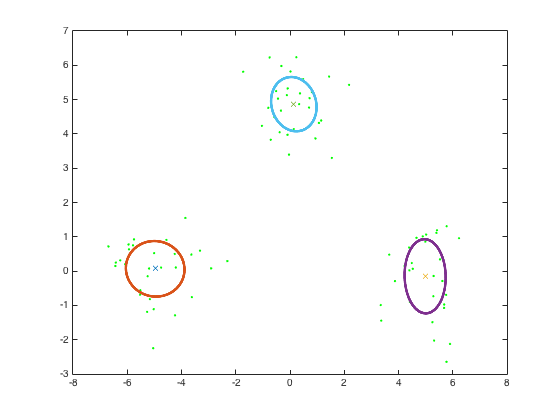
\includegraphics[width=0.75\linewidth]{figures/mixmodelA_3_20.png}
    \caption{Good fit on Dataset A with 3 GMM}
    \vspace{4ex}
  \end{subfigure}%%
  \begin{subfigure}[b]{0.5\linewidth}
  \centering
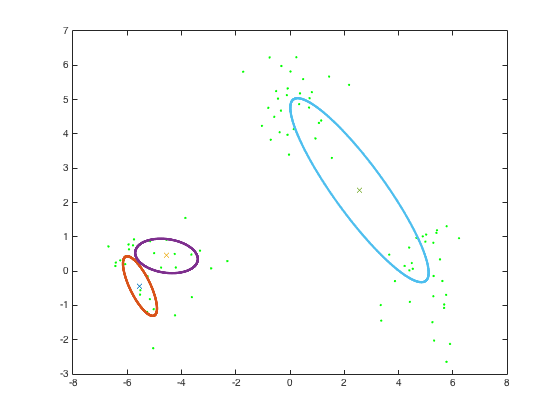
\includegraphics[width=0.75\linewidth]{figures/mixmodelA_3_500.png}
\caption{No good fit on Dataset A with 3 GMM}
\vspace{4ex}
\end{subfigure}%%
\end{figure}
%\verbatiminput{mixmodelA-3-20.txt}
\begin{figure}[ht]
\begin{subfigure}[b]{0.5\linewidth}
    \centering
    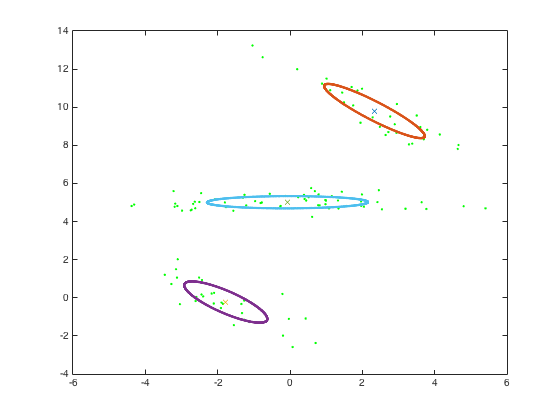
\includegraphics[width=0.75\textwidth]{figures/mixmodelB_3_20.png}
    \caption{Good fit on Dataset B with 3 GMM}
    \vspace{4ex}
 \end{subfigure}%%
  \begin{subfigure}[b]{0.5\linewidth}
  \centering
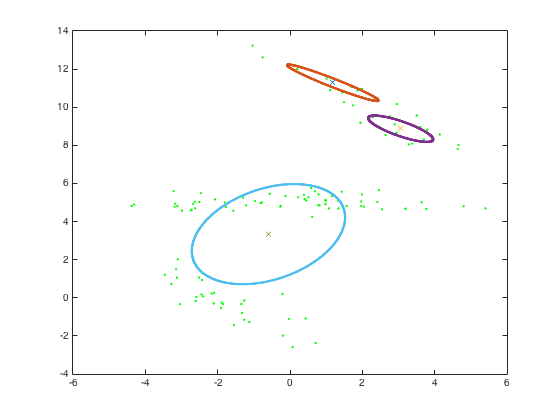
\includegraphics[width=0.75\linewidth]{figures/mixmodelB_3_500.png}
\caption{No good fit on Dataset B with 3 GMM}
\vspace{4ex}
\end{subfigure}%%
\end{figure}
The results of these experiments can be found in files \textit{mixmodelA-3-20.txt, mixmodelB-3-20.txt, mixmodelA-3-500.txt,
mixmodelB-3-500.txt}. The good fits are in 20 and the bad in 500. The numbers is the iteration I used.
%\verbatiminput{mixmodelB-3-20.txt}
\subsection*{Part B}
Doing Similar calculations with thw exercise 1 we are deriving the necessary
equations for the Bernoulli mixture models.
\begin{align*}
t_{n,k} &= \frac{\pi_{k}\mu_{k}^{x_{n}} (1-\mu_{k})^{1-x_{n}}}{\sum_{k'=1}^K \pi_{k'} \mu_{k'}^{x_{n}}(1-\mu_{k'})^{1-x_n}}\\
\mu_{k} &= \frac{\sum_{n=1}^N\sum_{i=1}^{D} t_{n,i}x_{n,i}}{D\sum_{n=1}^N t_{n,i}}\\
\pi_{k} &= \frac{\sum_{n=1}^{N}t_{n,k}}{\sum_{k'=1}^K\sum_{n=1}^{N}t_{n,k}}\\
L &= \sum_{n=1}^{N}\sum_{k=1}^{K}t_{n,k}(\sum_{i=1}^{D}x_{n,i}\log(\mu_{k})+(1-x_{n,i})(\log{1-\mu_{k}}) + \log\pi_{k})
\end{align*}
